% http://ena.lp.edu.ua:8080/bitstream/ntb/30105/1/17_96-103_Vis_573.pdf

\section{Проектування мультиагентної системи}
\subsection{Розробка вимог до програмної системи}
\subsubsection{Галузь застосування}
Даний програмний продукт може бути використаний логістичними компаніями з метою покращення сервісу, викладачами та студентами для дослідження логістичних систем.

\subsubsection{Бізнес вимоги}
Необхідно розробити програмний компонент для моделювання розподільчих логістичних систем різних конфігурацій з метою оцінки кожної з конфігурацій.

\subsubsection{Функціональні вимоги}
Специфікацію функціональних вимог у вигляді \acrshort{uml}-діаграми прецедентів представлено на рисунку~\ref{fig:system_usecase}.

\begin{figure}[H]
	\centering

	\tikzumlset{font=\footnotesize} 
	\tikzumlset{fill usecase=white}
	\begin{tikzpicture} 
		\umlactor[x=4, y=2]{Актор} 
		\umlusecase[x=1, y=0, width=3.5cm, name=service]{Перегляд параметрів системи у реальному часі} 
		\umlusecase[x=0, y=3, width=3.5cm, name=export]{Експорт конфігурації до \acrshort{json} файлу}

		\umlusecase[x=7, y=1, name=report]{Генерація звіту} 
		
		\umlusecase[x=11, y=5, name=report_c_period]{Вибір типу даних} 
		\umlusecase[x=9, y=3, name=report_c]{Конфігурація звіту} 
		\umlusecase[x=11, y=1, name=report_c_actors]{Вибір акторів}  

		\umlassoc{Актор}{service}
		\umlassoc{Актор}{export}
		\umlassoc{Актор}{report}

		\umlinclude{report}{report_c}
		\umlextend{report_c_period}{report_c}
		\umlextend{report_c_actors}{report_c}
	\end{tikzpicture}

	\caption{\acrshort{uml}-діаграма прецедентів системи}
	\label{fig:system_usecase}
\end{figure}

Список функціональних вимог системи:
\begin{enumerate}[label={\arabic*)}]
	\item система повинна мати можливість імпорту початкової конфігурації логістичної системи з \acrshort{json} файлу;
	\item система повинна автоматично приймати рішення о розподілі матеріальних потоків;
	\item система повинна мати графічний інтерфейс перегляду поточного стану логістичної системи: рівень запасу товарів, рівні сервісу, рівень ризику, навантаження мережі. 
	\item система повинна мати можливість генерації звіту.
\end{enumerate}

Генеруємий звіт та графічний інтерфейс програмної системи повинен включати (для кожній ітерації та агенту системи) рівень логістичного сервісу, перенапружені ланки логістичної системи, прогнозуємий рівень збиту, показники ризику.

\subsubsection{Нефункціональні вимоги}
Список нефункціональних вимог системи:
\begin{enumerate}[label={\arabic*)}]
	\item система повинна бути платформонезалежною та підтримувати такі операційні системи, як Debian, Windows, macOS;
	\item система повинна мати зручний інтерфейс;
	\item система повинна мати високий рівень зручності супроводу.
\end{enumerate}

\subsection{Модель вхідних данних}
В якості вхідних даних у система підтримує файли у форматі JSON з наданою нижче схемою: 

{\small
\begin{lstlisting}[language=json,firstnumber=1]
{
	"demand": [
		{
			"product": "tea",
			"vertex": "odessa",
			"sd": 0.005,
			"ev": 0.500
		},
	],
	"vertices": [
		{
			"type": "national|regional|local",
			"name": "odessa"
		}
	],
	"edges": [
		{
			"distance": 145.4,
			"from": "odessa",
			"to": "kyiv"
		}
	]
}
\end{lstlisting}
}

Альтернативна схема у вигляді діаграми класів представлена на рисунку~\ref{fig:arch_general_scheme}.

\begin{figure}[H]
	\centering
	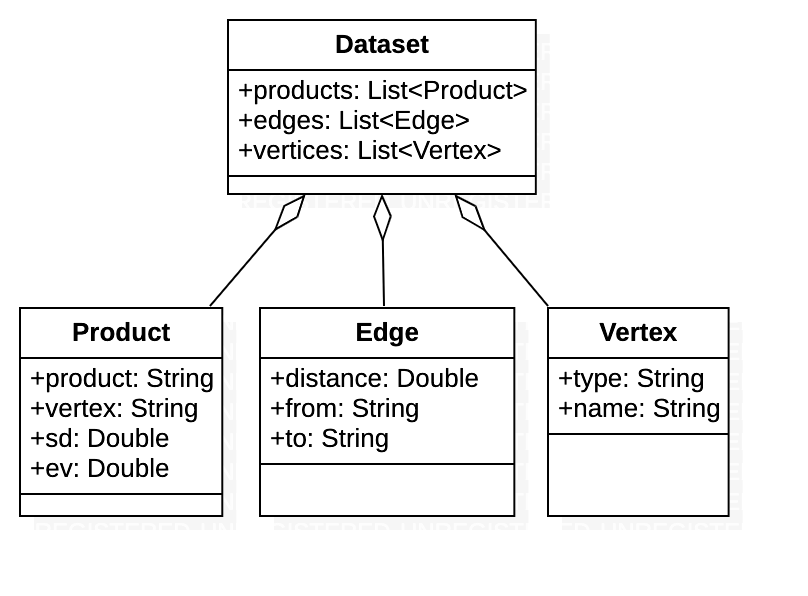
\includegraphics[width=0.7\textwidth]{arch_input_scheme}
	\caption{Схема вхідних даних}
	\label{fig:arch_input_scheme}
\end{figure}  

\subsection{Архітектура програмної системи}
\subsubsection{Аналіз та вибір агентної платформи}
Агентна платформа --- це проміжний виконавчий рівень, який знаходиться між агентами та операційною системою.
Існує велика кількість різноманітних агентних платформ, які значно спрощують розробку \acrshort{mas}~\cite{Kravari2015}.
При реалізації \acrshort{mas} можна виділити три основних підходи до розробки~\cite{Zhou2010}:
\begin{enumerate}[label={\arabic*)}]
	\item використання платформ розробки для побудови \acrshort{mas};
	\item програмування агентної системи за допомогою \acrshort{fipa} фреймворків;
	\item програмування агентної системи без використання фреймворків за допомогою загальних мов програмування.
\end{enumerate}

Головні засоби для розробки агентних систем наведено на рисунку~\ref{fig:arch_general_scheme}.

\begin{figure}[H]
	\centering
	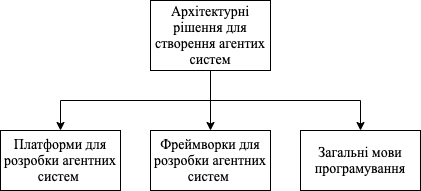
\includegraphics[width=0.75\textwidth]{arch_general_scheme}
	\caption{Засоби розробки агентних платформ}
	\label{fig:arch_general_scheme}
\end{figure} 

У таблиці~\ref{tab:mas_platform_comparsion} приведено порівняння різних підходів до розробки агентних платформ.

Платформи для розробки агентних систем (AnyLogic, AgentSheets та ін.) дозволяють швидко реалізувати модель агентой системи, мають обширну документацію та сервіси підтримки. Такі платформи підтримують однорівневу архітектуру. Недоліками використання готових платформ є їх висока ціна та обмежена гнучкість.

Фреймворки для розробки агентних систем (JADE, Agent Factory та ін.) реалізують комуникацію меж агентами та середу іх виконання. Такі фреймворки підтримують однорівневу та багаторівневі архітектури та дозволяють розміщувати агентів на різних фізичних машинах та використовувати різні фреймворки для різних агентів. Недоліками використання фрейморків є їх висока складність та складність супроводу через надмірну універсальність системи.

Використання загальних мов програмування для розробки агентних систем відчиняє доступ до обшірної колекції бібліотек та реалізацій алгорітмів для моделювання. Використання загальних мов програмування передбачає самостійне проектування та розробку архітектури системи без зайвих елементів. Такі системи легше супроводжувати та доповняти новим функціоналом. Недоліками є висока складність розробки.

Отже, для розробки було прийнято рішення писати свою легку платформу для запуску агентів через те, що готові фреймворки для побудови агентних систем мають надмірний функціонал та складні у використанні і вивченні.

\subsubsection{Компоненти програмної системи}
Розроблені варіанти компонентів архітектури програмної системи представлені на рисунках~\ref{fig:arch_component_v1} та~\ref{fig:arch_component_v2}.

\begin{figure}[H]
	\centering
	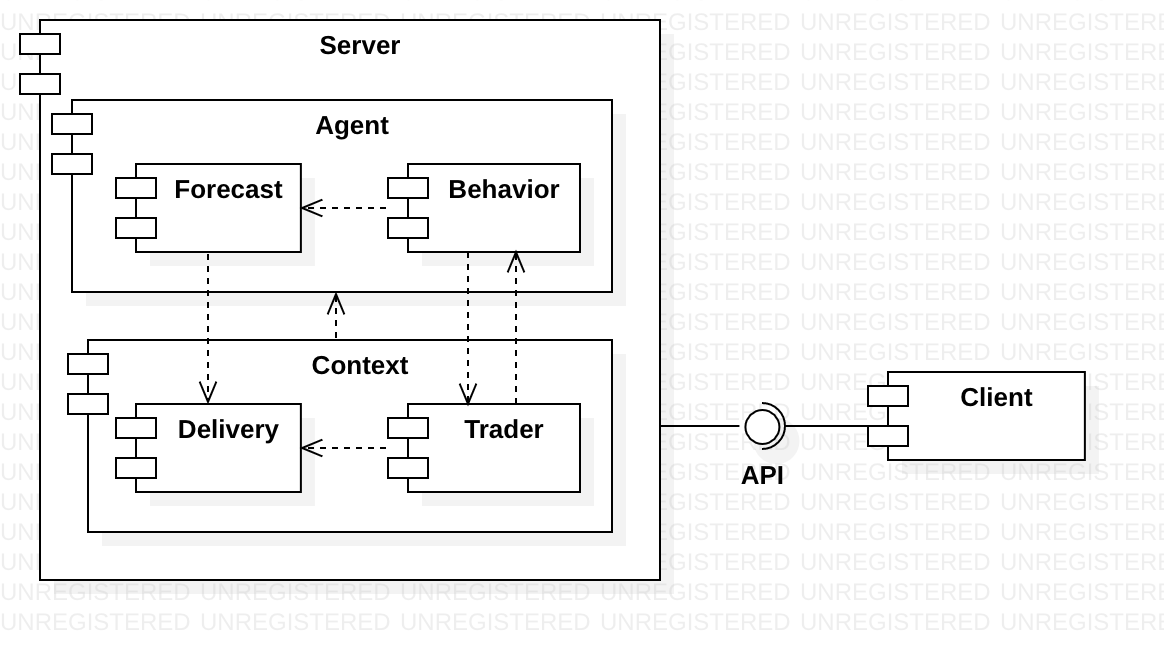
\includegraphics[width=0.85\textwidth]{arch_component_v1}
	\caption{Модель компонентів централізованої системи}
	\label{fig:arch_component_v1}
\end{figure} 

\begin{figure}[H]
	\centering
	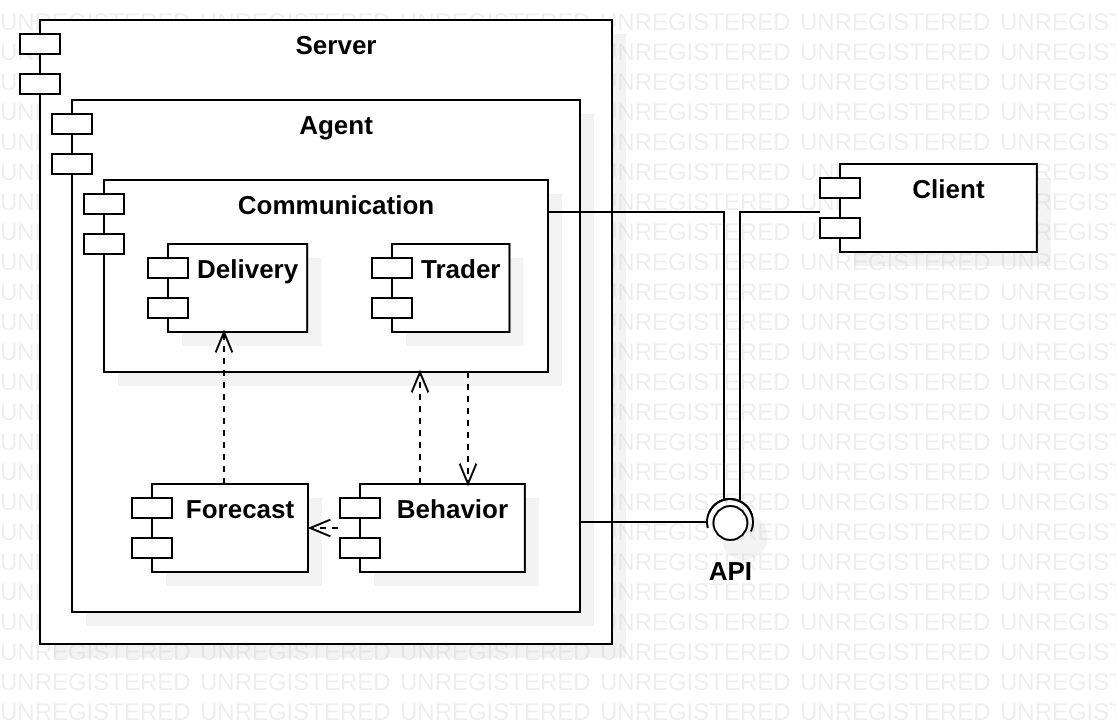
\includegraphics[width=0.85\textwidth]{arch_component_v2}
	\caption{Модель компонентів децентралізованої системи}
	\label{fig:arch_component_v2}
\end{figure} 

Основні проблеми реалізації децентралізованої архітектури обумовлені складністю комунікацїї між компонентами системи. Децентралізовані системи потребують значних людських ресурсів на реалізацію протоколів комуникацїї та додаткових обчислювальних ресурсів на комунікацїю між різними агентами.
Перевагами децентралізованих систем є висока відмовостійкість та масштабованість.
Перевагами централізованих систем є висока швидкість роботи, простота розробки.

Для реалізації системи була обрана централізована архітектура системи. 
Головною причинами вибору є недолік людських ресурсів та те, що моделювання буде проводитися на окремій машині з налаштованою системою, а отже масштабованість менш важлива ніж обчіслювальна потужність та складність розробки.    

Більш детально діаграма компонентів представлена на рисунку~\ref{fig:arch_component}.

\begin{figure}[H]
	\centering
	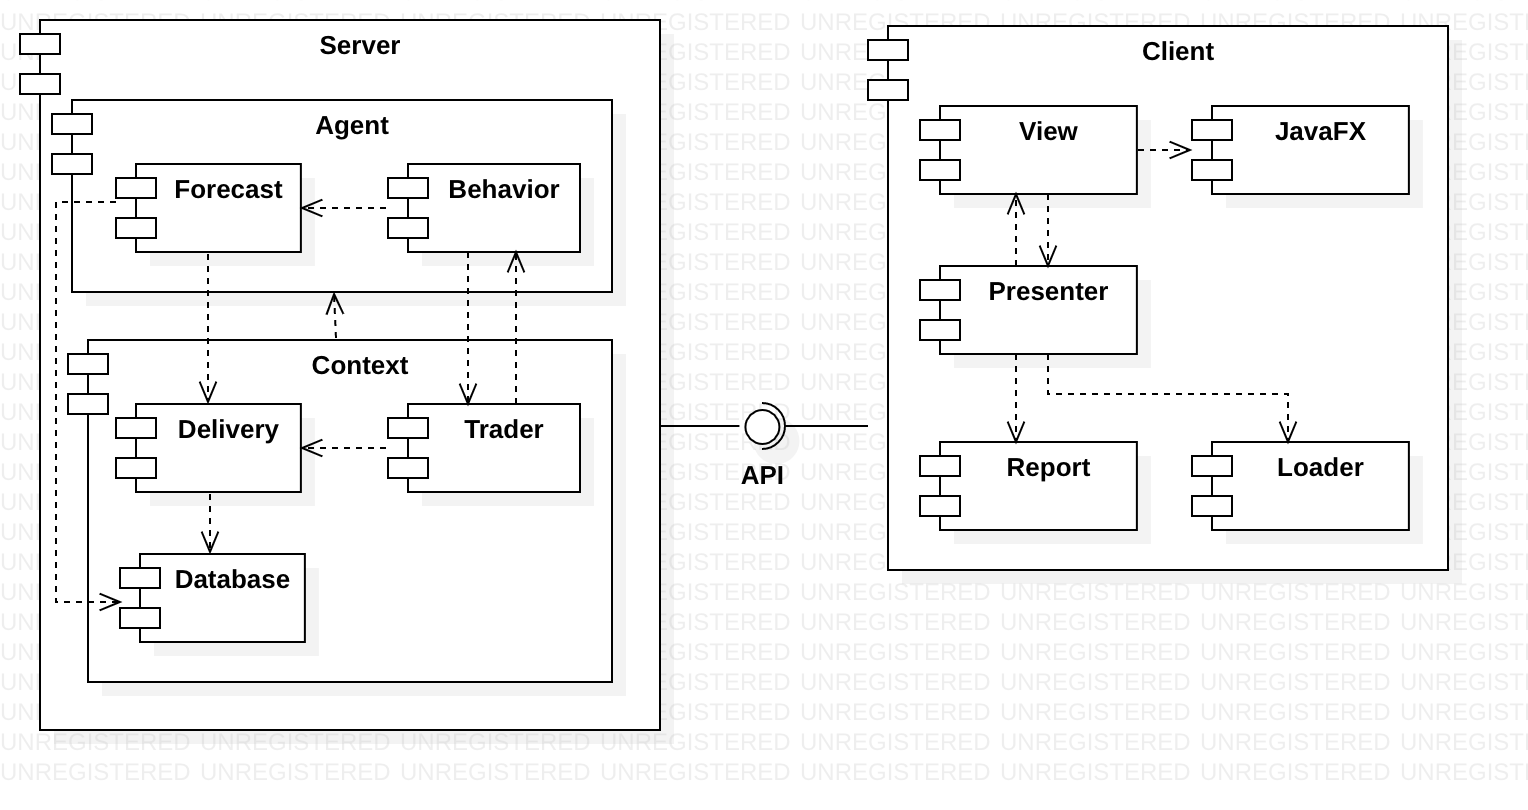
\includegraphics[width=\textwidth]{arch_component}
	\caption{Модель компонентів системи}
	\label{fig:arch_component}
\end{figure} 

Головними компонентами є:
\begin{itemize}
	\item \texttt{Server} --- платформа для асинхронного запуску та взаємодії агентів;
	\begin{itemize}
		\item \texttt{Context} --- навколишня середа агентів:
		\begin{itemize}
			\item \texttt{Database} --- сервіс бази даних, який зберігає всю інформацію про минулі рівні попиту та рівні сервісу;  
			\item \texttt{Delivery} --- сервіс розрахунку коштів доставки та доставки товарів від агента до агента;
			\item \texttt{Trader} --- сервіс укладення угод купівлі/продажу між агентами.
		\end{itemize}
		\item \texttt{Agent} --- компомент, який реалізує актора розподільчої логістичної системи:
		\begin{itemize}
			\item \texttt{Forecast} --- компонент прогнозування запасів агента;
			\item \texttt{Behavior} --- компонент логіки агента.
		\end{itemize}
	\end{itemize}
	\item \texttt{Client} --- графічний інтерфейс користувача;
	\begin{itemize}	
		\item \texttt{Presenter} --- компонент для взаємодії між інтерфейсом користувача та агентною платформою.
		\item \texttt{View} --- графічний інтерфейс користувача;
		\item \texttt{Report} --- створення звіту;
		\item \texttt{Loader} --- компонент для запису та читання з файлів.
	\end{itemize}
\end{itemize}

\subsubsection{Діаграма розгортання}
На рисунку~\ref{fig:arch_deployment} зображена запропонована для реалізації у програмній компоненті двохрівнева архітектура з тонким клієнтом.

\begin{figure}[H]
	\centering
	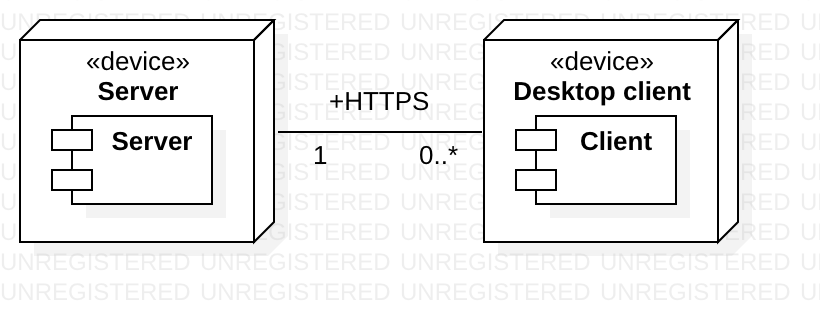
\includegraphics[width=0.75\textwidth]{arch_deployment}
	\caption{\acrshort{uml}-діаграма розгортування системи}
	\label{fig:arch_deployment}
\end{figure} 

\subsubsection{Діаграма класів}
На рисунку~\ref{fig:system_class} зображена діаграма класів системи.

\begin{figure}[H]
	\centering
	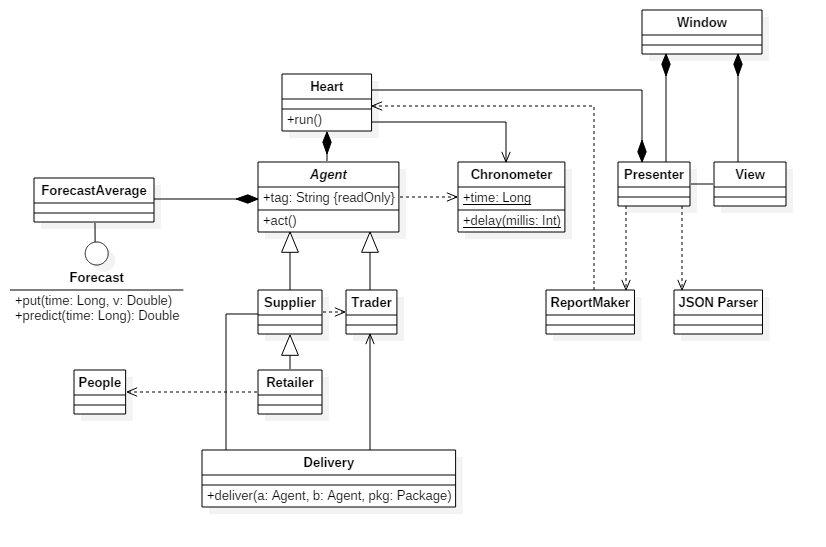
\includegraphics[width=\textwidth]{system_class}
	\caption{\acrshort{uml}-діаграма класів системи}
	\label{fig:system_class}
\end{figure} 

Головними класами є:
\begin{itemize}
	\item \texttt{Heart} --- керує асинхронним запуском та взаємодією агентів;
	\item \texttt{Agent} --- базовий клас який не має поведінки;
	\item \texttt{Supplier} --- агент-постачальник;
	\item \texttt{Retailer} --- агент-роздрібний-продавець;
	\item \texttt{Delivery} --- сервіс доставки замовлень;
	\item \texttt{Trader} --- агент-трейдер, який керує активними тендерами;
	\item \texttt{Observer} --- слідкує за поточним станом агентів та надає інформацію про них;
	\item \texttt{Chronometer} --- операції з поточним часом системи;
	\item \texttt{ForecastAverage} --- прогнозування методом ковзної середньої.
\end{itemize}

\subsubsection{Діаграма послідовності}
На рисунку~\ref{fig:arch_seq_warehouse_ask} зображена діаграма послідовності розміщення замовлення агентом складу, та опис кожної дії.

\begin{figure}[H]
	\centering
	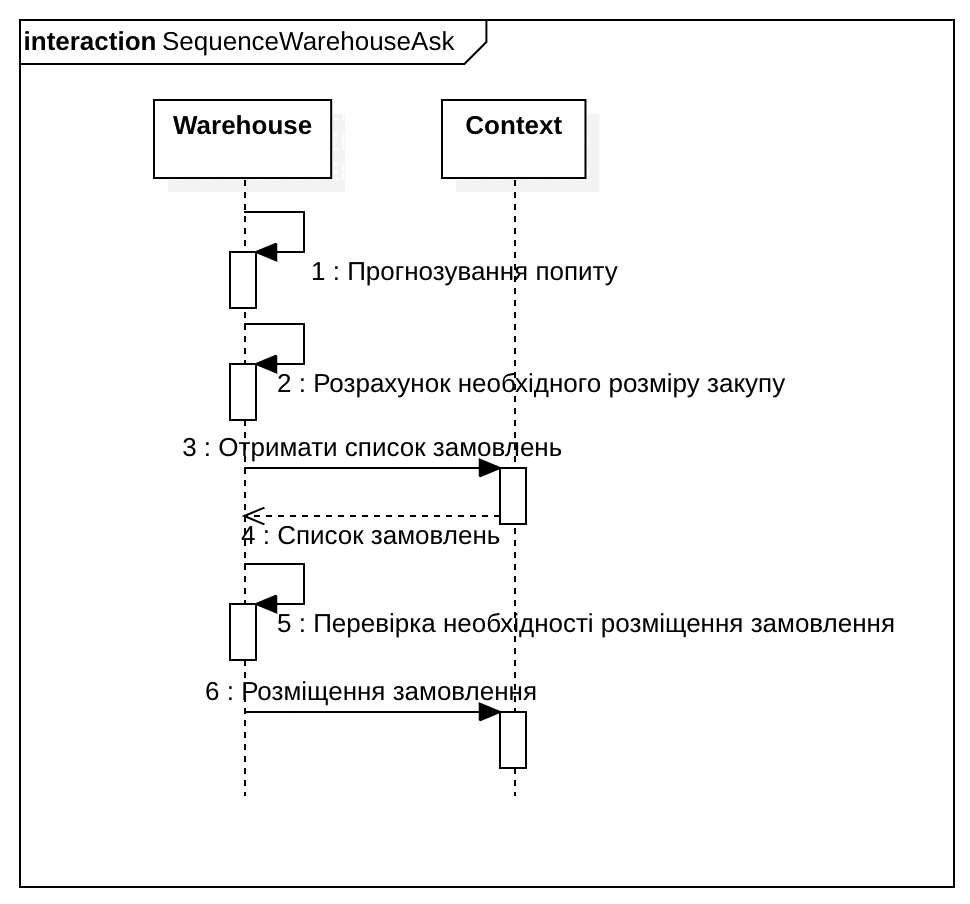
\includegraphics[width=0.7\textwidth]{arch_seq_warehouse_ask}
	\caption{\acrshort{uml}-діаграма послідовності}
	\label{fig:arch_seq_warehouse_ask}
\end{figure} 

На діаграмі позначено:
\begin{itemize}
	\item Агент складу виконує операцію прогнозування попиту.
	\item Агент складу розраховує необхідний розмір закупу товарів.
	\item Агент складу запрошує список замовлень, що існують у даний момент часу.
	\item Агент складу отримує список замовлень.
	\item Агент складу перевіряє необхідність розміщення замовлення. 
	\item Агент складу розміщує замовлення на поповнення запасу.
\end{itemize}

На рисунку~\ref{fig:arch_seq_demand} зображена діаграма послідовності агенту попиту, та опис кожної дії.

\begin{figure}[H]
	\centering
	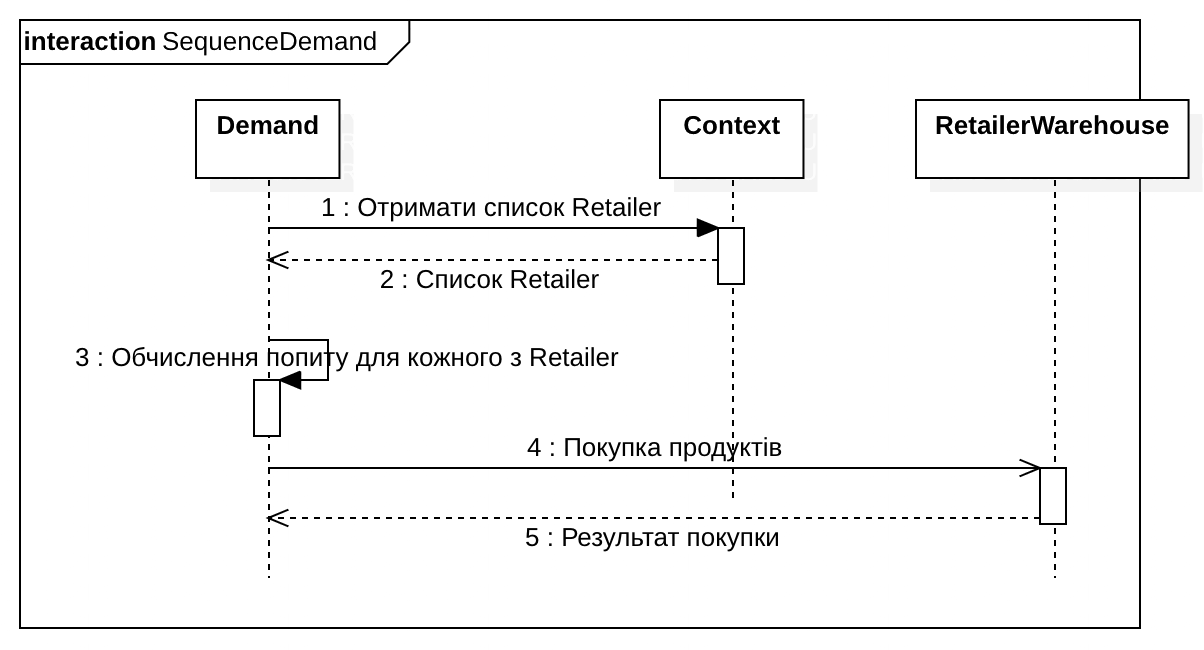
\includegraphics[width=0.8\textwidth]{arch_seq_demand}
	\caption{\acrshort{uml}-діаграма послідовності}
	\label{fig:arch_seq_demand}
\end{figure} 

На діаграмі позначено:
\begin{itemize}
	\item Агент попиту запрошує список роздрібних продавців.
	\item Агент попиту отримує список роздрібних продавців.
	\item Агент обчислює попит для кожного роздрібного продавця.
	\item Агент імітує покупку продуктів у роздрібних продавців.
\end{itemize}

На рисунку~\ref{fig:arch_seq_warehouse_send} зображена діаграма послідовності розміщення пропозиції доставки агентом складу, та опис кожної дії.

\begin{figure}[H]
	\centering
	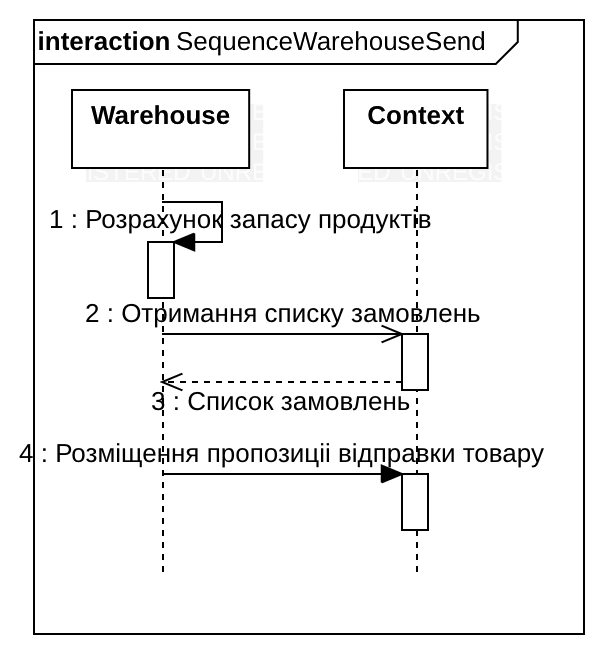
\includegraphics[width=0.45\textwidth]{arch_seq_warehouse_send}
	\caption{\acrshort{uml}-діаграма послідовності}
	\label{fig:arch_seq_warehouse_send}
\end{figure} 

На діаграмі позначено:
\begin{itemize}
	\item Агент складу виконує розрахунок запасу продуктів.
	\item Агент складу запрошує список замовлень від обслуговуємих агентів.
	\item Агент складу отримує список замовлень.
	\item Агент складу розміщує пропозицію відправки товару.
\end{itemize}

На рисунку~\ref{fig:arch_seq_warehouse_choose} зображена діаграма послідовності вибору вигідної пропозиції та запрошення створення контракту на доставку товару, та опис кожної дії.

\begin{figure}[H]
	\centering
	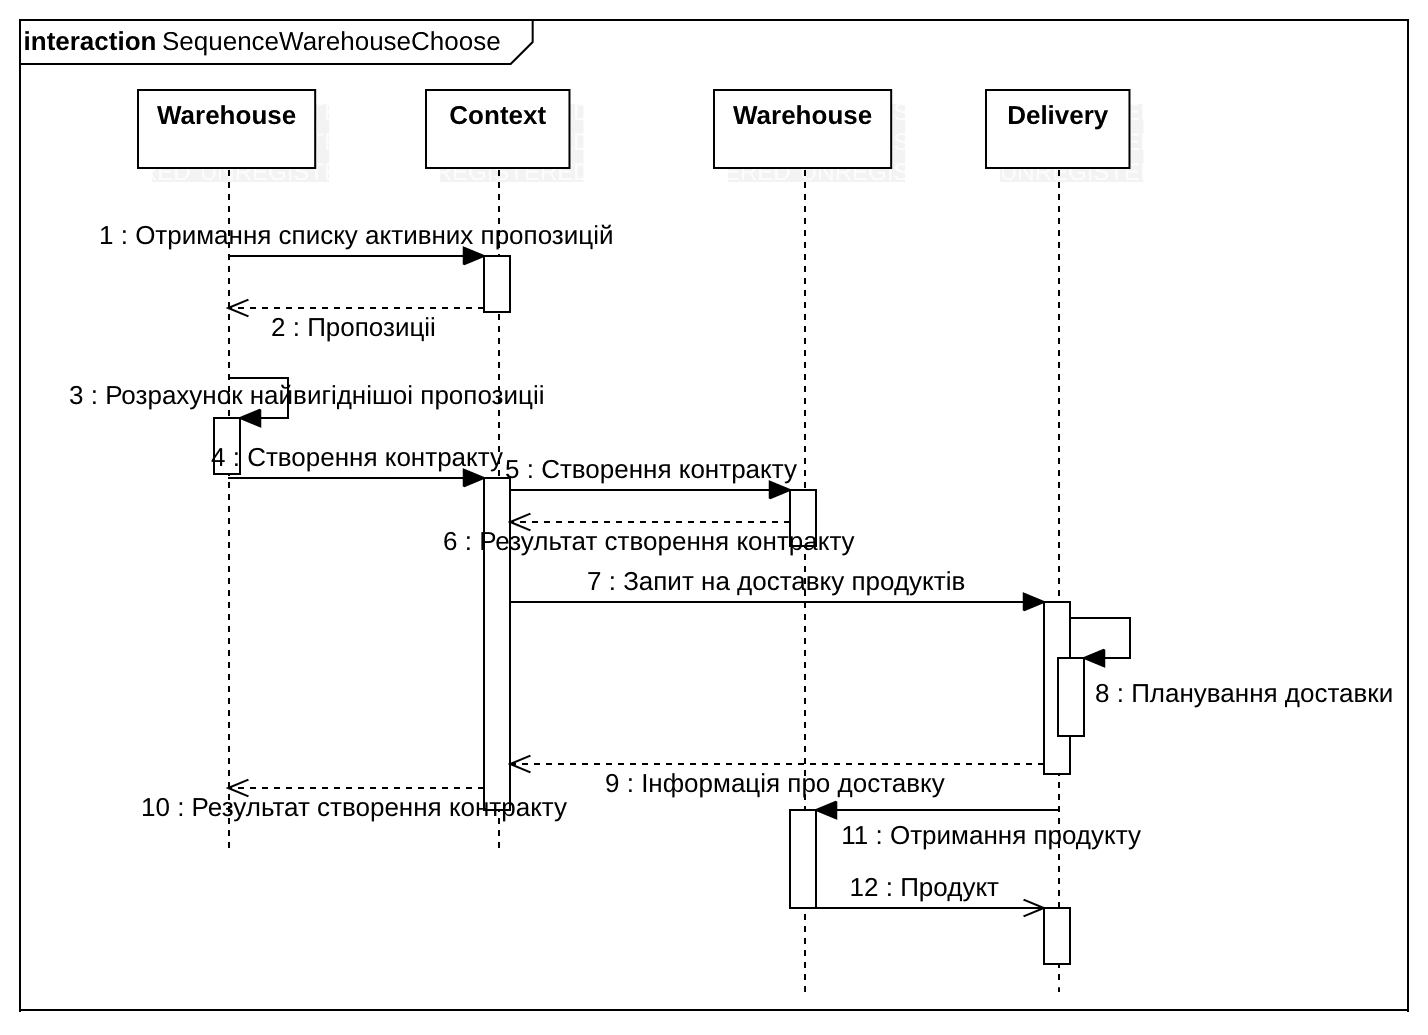
\includegraphics[width=\textwidth]{arch_seq_warehouse_choose}
	\caption{\acrshort{uml}-діаграма послідовності}
	\label{fig:arch_seq_warehouse_choose}
\end{figure} 

На діаграмі позначено:
\begin{itemize}
	\item Агент-замовник запрошує список активних пропозицій.
	\item Агент-замовник отримує список активних пропозицій.
	\item Агент-замовник розраховує найвигіднішу пропозицію.
	\item Агент-замовник запрошує створення контракту з агентом-
	постачальником.
	\item Агент-постачальник отримує запит на створення контракту.
	\item Агент-постачальник підтверджує створення контракту.
	\item Агент-постачальник робить запит на доставку товару у агента
	доставки.
	\item Агент доставки планує доставку.
	\item Агент доставки передає інформацію про доставку.
	\item Агент-замовник отримує результат створення контракту.
	\item Агент доставки запрошує у агент-постачальника товари для
	доставки.
	\item Агент-постачальник передає товари для доставки агенту доставки.
\end{itemize}

На рисунку~\ref{fig:arch_seq_warehouse_receive} зображена діаграма послідовності доставки товару та закриття контракту, та опис кожної дії.

\begin{figure}[H]
	\centering
	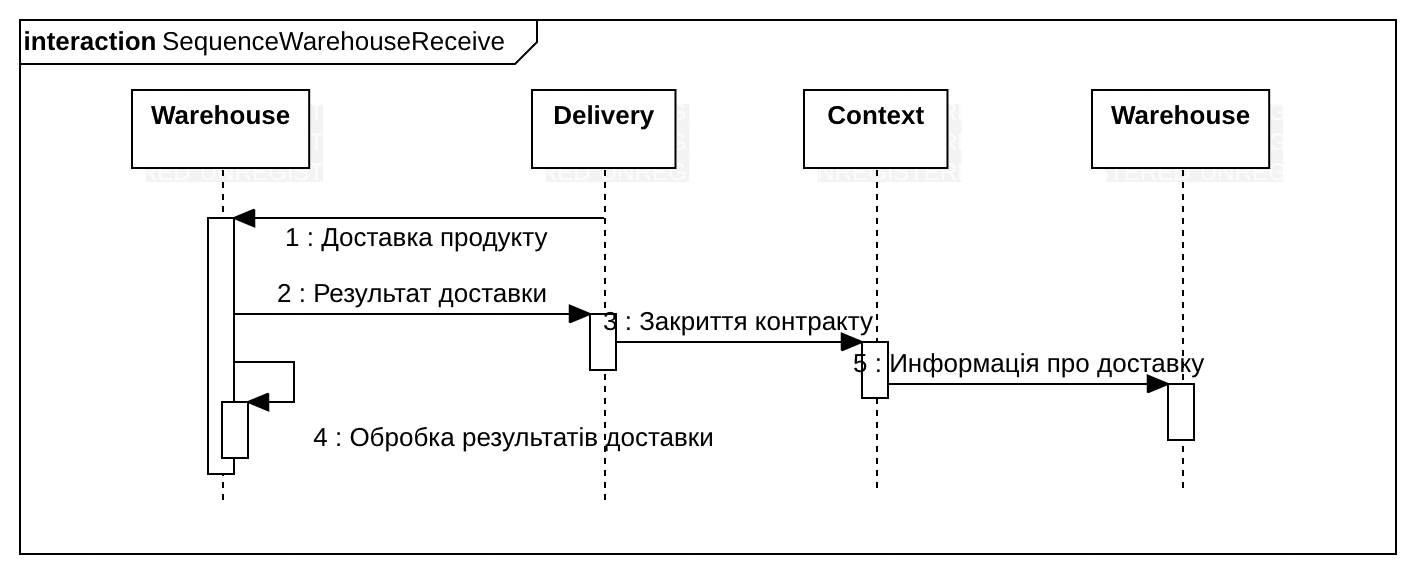
\includegraphics[width=\textwidth]{arch_seq_warehouse_receive}
	\caption{\acrshort{uml}-діаграма послідовності}
	\label{fig:arch_seq_warehouse_receive}
\end{figure} 

На діаграмі позначено:
\begin{itemize}
	\item Агент доставки передає замовлені товари агенту-замовнику.
	\item Агент замовник підтверджує доставку товарів.
	\item Агент доставки закриває контракт доставки.
	\item Агент-постачальника проінформовано про результат контракту. 
	\item Агент-замовник обробляє результат доставки.
\end{itemize}

Спрощена діаграма послідовності всієї системи представлена на рисунку~\ref{fig:arch_seq}.

\begin{figure}[H]
	\centering
	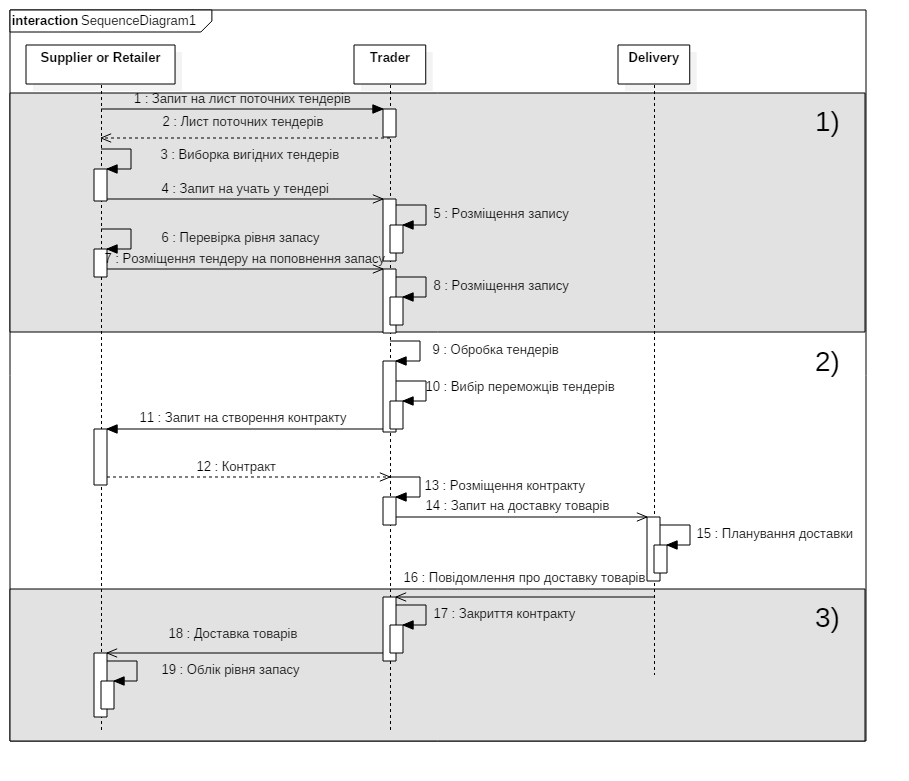
\includegraphics[width=\textwidth]{arch_seq}
	\caption{\acrshort{uml}-діаграма послідовності}
	\label{fig:arch_seq}
\end{figure} 

\begin{enumerate}[label={\arabic*)}]
	\item спрощений життєвий цикл постачальника та роздрібного торговця;
	\item спрощений життєвий цикл трейдера;
	\item спрощений життєвий цикл системи доставки.
\end{enumerate}

\subsubsection{Діаграми активності}
На рисунку~\ref{fig:system_retailer_activity} зображена діаграма активності життєвого циклу роздрібного продавця.

\begin{figure}[H]
	\centering
	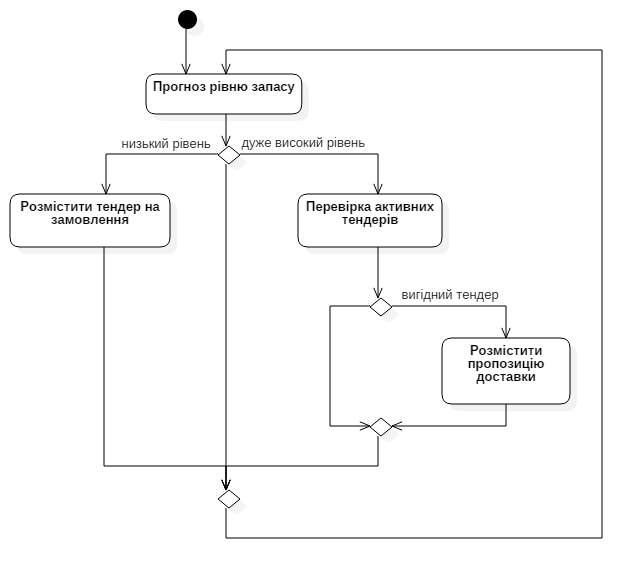
\includegraphics[width=0.75\textwidth]{system_retailer_activity}
	\caption{\acrshort{uml}-діаграма активності життєвого циклу роздрібного продавця}
	\label{fig:system_retailer_activity}
\end{figure} 

\subsection{Обґрунтування вибору інструментальних засобів}
\subsubsection{Мова програмування Kotlin}
Основна мета мови Kotlin --- запропонувати більш компактну, продуктивну і безпечну альтернативу мови Java, придатну для використання всюди, де сьогодні використовується Java.
Kotlin чудово підходить для розробки серверних застосунків, дозволяя писати стислий та експресивний код.
Переваги Kotlin~\cite{kotlin,Panchal2017}:  
\begin{enumerate}[label={\arabic*)}]
	\item експресивність --- інноваційні можливості Kotlin, такі як типо-безпечні конструктори та делегати, дозволяють створювати потужні та прості у використанні абстракції;
	\item масштабованість --- підтримка Kotlin корутин \textit{(coroutines)} допомагає створювати масштабовані застосунки;
	\item сумістність --- Kotlin повністю сумісний зі всіма Java фреймворками;
	\item міграція --- Kotlin підтримує покроковий перехід з кодової бази на Java;
	\item інструменти --- Kotlin добре підтримується середовищами програмування;
	\item легкість навчання --- для Java розробника дуже легко почати вивчати Kotlin.
\end{enumerate}

\subsubsection{Система управління версіями Git}
Використання системи контролю версії є необхідним для роботи над великими проектами.

Система контролю дозволяє зберігати попередні версії файлів та завантажувати їх за потребою. 
Вона зберігає повну інформацію про версію кожного з файлів, а також повну структуру проекту на всіх стадіях розробки.

Git --- розподілена система керування версіями файлів та спільної роботи. Git є однією з найефективніших, надійних і високопродуктивних систем керування версіями, що надає гнучкі засоби нелінійної розробки, що базуються на відгалуженні і злитті гілок~\cite{Chacon2009}.

\subsubsection{Середовище розробки застосунків Intellij IDEA}
IntelliJ IDEA --- інтегроване середовище розробки програмного забезпечення багатьма мовами програмування. 
Community версія середовища IntelliJ IDEA підтримує інструменти для проведення тестування TestNG і JUnit, системи контролю версій CVS, Subversion, Mercurial і Git, засоби збирання Maven і Ant, мови програмування Kotlin, Java, Java ME, Scala, Clojure і Groovy. 
Середовище містить редактор регулярних виразів, систему перевірки коректності коду, система контролю за виконанням завдань та ін.~\cite{Kalinichenko2013}.

Середовище IntelliJ IDEA є рекомендованим для розробки застосунків на мові програмування Kotlin~\cite{kotlin}.

